Our image captioning model is summarized in Figure \ref{img:cap_frame}. The model includes an image analysis part and a caption generation part. In the image analysis part, we first use supervised learning to predict a set of attributes, based on words commonly found in image captions %
We solve this as a \textit{multi-label classification problem} and train a corresponding deep CNN by minimizing an element-wise logistic loss function. Secondly, a fixed length vector $\Att(I)$ is created for each image $I$, whose length is the size of the attribute set. Each dimension of the vector contains the prediction probability for a particular attribute. In the captioning generation part, we apply an LSTM-based sentence generator. In the baseline model, as in~\cite{gao2015you,ren2015image,vinyals2014show} we use a pre-trained CNN to extract image features $\CNN(I)$ which are fed into the LSTM directly. For the sake of completeness a fine-tuned version of this approach is also implemented.

\subsection{Attribute-based Image Representation}
\label{subsec:Attributes_Predictor}
Our first task is to describe the image content in terms of a set of attributes. An attribute vocabulary is first constructed. Unlike~\cite{kulkarni2013babytalk,yang2011corpus}, that use a vocabulary from separate hand-labeled training data, our semantic attributes are extracted from training captions and can be any part of speech, including object names (nouns), motions (verbs) or properties (adjectives). The direct use of captions guarantees that the most salient attributes for an image set are extracted. We use the $c$ ($c=256$) most common words in the training captions to determine the attribute vocabulary $\mathcal{V}_{att}$. Similar to \cite{fang2014captions}, the top $15$ most frequent closed-class words such as \texttt{`a',`on',`of'}  are removed since they are in nearly every caption. In contrast to~\cite{fang2014captions}, our vocabulary is not tense or plurality sensitive, for instance, \texttt{`ride'} and \texttt{`riding'} are classified as the same semantic attribute, similarly \texttt{`bag'} and \texttt{`bags'}. This significantly decreases the size of our attribute vocabulary. The full list of attributes can be found in the supplementary material. Our attributes represent a set of high-level semantic constructs, the totality of which the LSTM then attempts to represent in sentence form. Generating a sentence from a vector of attribute likelihoods exploits a much larger set of candidate words which are learned separately, allowing for greater flexibility in the generated text.

Given this attribute vocabulary, we can associate each image with a set of attributes according to its captions. We then wish to predict the attributes given a test image. Because we do not have ground truth bounding boxes for attributes, we cannot train a detector for each using the standard approach. Fang \etal~\cite{fang2014captions} solved a similar problem using a Multiple Instance Learning framework~\cite{zhang2005multiple} to detect visual words from images. Motivated by the relatively small number of times that each word appears in a caption, we instead treat this as a multi-label classification problem. To address the concern that some attributes may only apply to image sub-regions, we follow Wei \etal~\cite{wei2014cnn} in designing a region-based multi-label classification framework that takes an arbitrary number of sub-region proposals as input, then a shared CNN is associated with each proposal, and the CNN output results from different proposals are aggregated with max pooling to produce the final prediction.

Figure \ref{img:attributes} summarizes the attribute prediction network. The model is a VggNet structure followed by a max-pooling operation on the regions with a multi-label loss. The CNN model is first initialized from the VggNet pre-trained on ImageNet.
%
The shared CNN is then fine-tuned on the target multi-label dataset (our image-attribute training data). In this step, the input is the global image and the output of the last fully-connected layer is fed into a $c$-way softmax over the $c$ class labels. The $c$ here represents the attributes vocabulary size. In contrast to \cite{wei2014cnn} who employs the squared loss, we find that element-wise logistic loss function performs better. Suppose that there are $N$ training examples and $\bm{y_i}=[y_{i1}, y_{i2},... , y_{ic}]$ is the label vector of the $i^{th}$ image, where $y_{ij}=1$ if the image is annotated with attribute $j$, and $y_{ij}=0$ otherwise. If the predictive probability vector is $\bm{p_i}=[p_{i1}, p_{i2},... , p_{ic}]$, the cost function to be minimized is
\begin{equation}
 J=\frac{1}{N}\sum_{i=1}^{N}\sum_{j=1}^{c}\log(1+\exp(-y_{ij}p_{ij}))
\end{equation}
During the fine-tuning process, the parameters of the last fully connected layer (i.e. the attribute prediction layer) are initialized with a Xavier initialization \cite{glorot2010understanding}. The learning rates of  `\texttt{fc6}' and `\texttt{fc7}' of the VggNet are initialized as 0.001 and the last fully connected layer is initialized as 0.01. All the other layers are fixed during training. We executed 40 epochs in total and decreased the learning rate to one tenth of the current rate for each layer after 10 epochs. The momentum is set to 0.9. The dropout rate is set to 0.5.

To predict attributes based on regions, we first extract hundreds of proposal windows from an image. However, considering the computational inefficiency of deep CNNs, the number of proposals processed needs to be small. Similar to \cite{wei2014cnn}, we first apply the normalized cut algorithm to group the proposal bounding boxes into $m$ clusters based on the IoU scores matrix. The top $k$ hypotheses in terms of the predictive scores reported by the proposal generation algorithm are kept and fed into the shared CNN. We also include the whole image in the hypothesis group. As a result, there are $mk+1$ hypotheses for each image. We set $m=10, k=5$ in all experiments. We use Multiscale Combinatorial Grouping (MCG)~\cite{PABMM2015} for the proposal generation. Finally, a cross hypothesis max-pooling is applied to integrate the outputs into a single prediction vector $\Att(I)$.

Since we formulate the attribute prediction as a multi-label problem, our attributes prediction network can be replaced by any other multi-label classification framework and it also can be benefit from the development of the multi-label classification researches. For example, to address the computational inefficiency of using a large numbers of proposed regions, we can apply an `R-CNN' architecture~\cite{girshick2015fast} so that we do not need to compute the convolutional feature map multiple times. The Regional Proposal Network~\cite{ren2015faster} can predict region proposal and attributes together so that we do not need the external region proposal tools. We even can consider the attributes dependencies by using the recently proposed CNN-RNN model \cite{wang2016cnn}. However, we leave them as the further work.

\begin{figure}[t!]
  \centering
  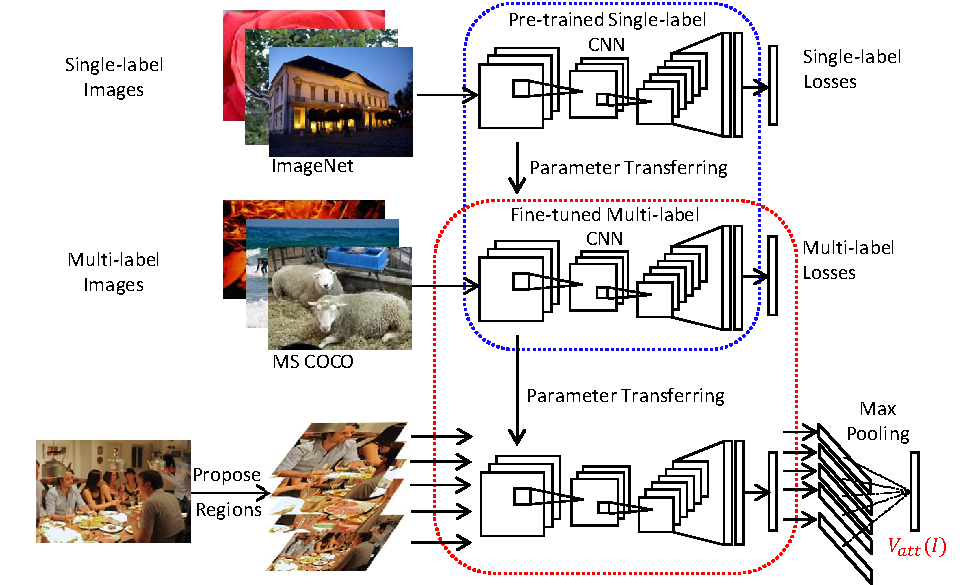
\includegraphics[width=1\linewidth]{./img/attributes_layer.pdf}\\
  \caption{Attribute prediction CNN: the model is initialized from VggNet~\cite{simonyan2014very} pre-trained on ImageNet. The model is then fine-tuned on the target multi-label dataset. Given a test image, a set of proposal regions are selected and passed to the shared CNN, and finally the CNN outputs from different proposals are aggregated with max pooling to produce the final multi-label prediction, which gives us the high-level image representation, $\Att(I)$}
  \label{img:attributes}
  \vspace{-10pt}
\end{figure}

\subsection{Caption Generation Model}
\label{subsec:caption_model}
Similar to~\cite{Karpathy2014deepvs,mao2014deep,vinyals2014show}, we propose to train a caption generation model by maximizing the probability of the correct description given the image. However, rather than using image features directly as in typically the case, we use the semantic attribute prediction value $\Att(I)$ from the previous section as the input. Suppose that $\{S_1,...,S_L\}$ is a sequence of words. The log-likelihood of the words given their context words and the corresponding image can be written as:
\begin{equation}
    \log p(S|\Att(I))=\sum_{t=1}^L \log p(S_{t}|S_{1:t-1},\Att(I))
\end{equation}
where $p(S_t|S_{1:t-1},\Att(I))$ is the probability of generating the word $S_t$ given attribute vector $\Att(I)$ and previous words $S_{1:t-1}$. We employ the LSTM \cite{hochreiter1997long}, a particular form of RNN, to model this.

The LSTM is a memory cell encoding knowledge at every time step for what inputs have been observed up to this step. We follow the model used in \cite{zaremba2014learning}. Letting $\sigma$ be the sigmoid nonlinearity, the LSTM updates for time step $t$ given inputs $x_t$, $h_{t-1}$, $c_{t-1}$ are:

\vspace{-10pt}
\begin{eqnarray}
  i_t &=& \sigma(W_{xi}x_t+W_{hi}h_{t-1}+b_i) \\
  f_t &=& \sigma(W_{xf}x_t+W_{hf}h_{t-1}+b_f) \\
  o_t &=& \sigma(W_{xo}x_t+W_{ho}h_{t-1}+b_o) \\
  g_t &=& \tanh(W_{xc}x_t+W_{hc}h_{t-1}+b_c) \\
  c_t &=& f_t\odot c_{t-1}+i_t\odot g_t \\
  h_t &=& o_t \odot \tanh(c_t) \\
  p_{t+1} &=& {\rm softmax}(h_t)
\end{eqnarray}

Here, $i_t, f_t, c_t, o_t$ are the input, forget, memory, output state of the LSTM. The various $W$ matrices are trained parameters and $\odot$ represents the product with a gate value. $h_t$ is the hidden state at time step $t$ and is fed to a Softmax, which will produce a probability distribution $p_{t+1}$ over all words and indicate the word at time step $t+1$.

\vspace{3pt}
\noindent \textbf{Training details:} The LSTM model for image captioning is trained in an unrolled form. More formally, the LSTM takes the attributes vector $\Att(I)$ and a sequence of words $S=(S_0,...,S_L,S_{L+1})$, where $S_0$ is a special start word and $S_{L+1}$ is a special END token. Each word has been represented as a one-hot vector $S_t$ of dimension equal to the size of words dictionary. The words dictionaries are built based on words that occur at least 5 times in the training set, which lead to 2538, 7414, and 8791 words on Flickr8k, Flickr30k and MS COCO datasets separately. Note it is different from the semantic attributes vocabulary $\mathcal{V}_{att}$. The training procedure is as following: At time step $t=-1$, we set $x_{-1}=W_{ea}\Att(I)$, $h_{initial}=\vec{0}$ and $c_{initial}=\vec{0}$, where $W_{ea}$ is the learnable attributes embedding weights. This gives us an initial LSTM hidden state $h_{-1}$ which can be used in the next time step. From $t=0$ to $t=L$, we set $x_t=W_{es}S_t$ and the hidden state $h_{t-1}$ is given by the previous step, where $W_{es}$ is the learnable word embedding weights. The probability distribution $p_{t+1}$ over all words is then computed by the LSTM feed-forward process. Finally, on the last step when $S_{L+1}$ represents the last word, the target label is set to the END token.

\begin{figure}[t]
\begin{center}
   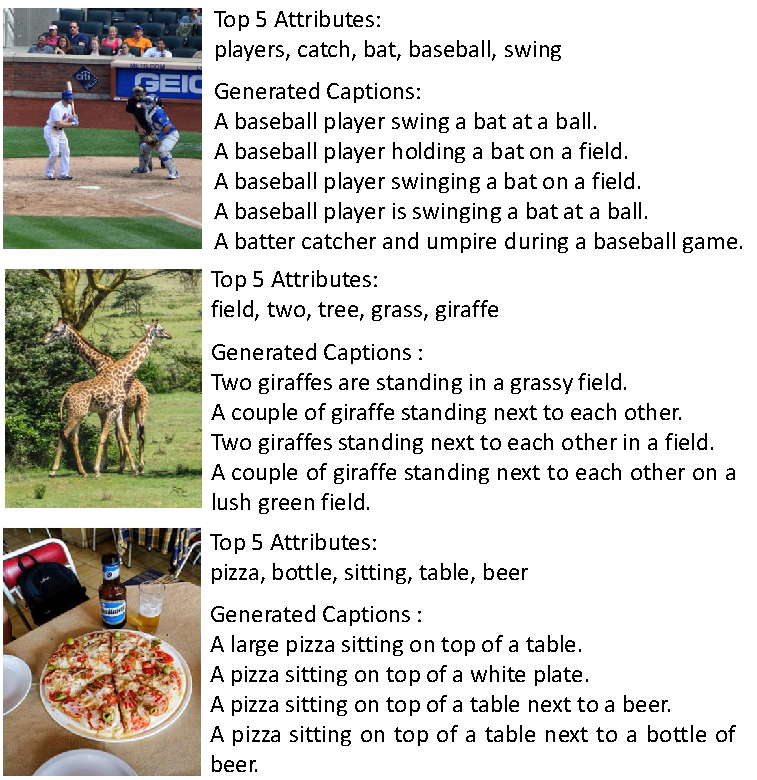
\includegraphics[width=0.95\linewidth]{img/samples_3.pdf}
\end{center}
\vspace{-10pt}
   \caption{Examples of predicted attributes and generated captions.}
   \vspace{-7pt}
   \label{att_caP_examples}
\end{figure}

Our training objective is to learn parameters $W_{ea}$, $W_{es}$ and all parameters in LSTM by minimizing the following cost function:
\begin{eqnarray}
    \mathcal{C}&=&-\frac{1}{N}\sum_{i=1}^N\log p(S^{(i)}|\Att(I^{(i)}))+\lambda_\ModParms\cdot||\ModParms||_2^2 \\
    &=&-\frac{1}{N}\sum_{i=1}^N\sum_{t=1}^{L^{(i)}+1}\log p_t(S_t^{(i)})+\lambda_\ModParms\cdot||\ModParms||_2^2
    \vspace{-3pt}
\end{eqnarray}
where $N$ is the number of training examples and $L^{(i)}$ is the length of the sentence for the $i$-th training example. $p_t(S_t^{(i)})$ corresponds to the activation of the Softmax layer in the LSTM model for the $i$-th input and $\ModParms$ represents model parameters, $\lambda_\ModParms\cdot||\ModParms||_2^2$ is a regularization term. We use SGD with mini-batches of 100 image-sentence pairs. The attributes embedding size, word embedding size and hidden state size are all set to 256 in all the experiments. The learning rate is set to 0.001 and clip gradients is 5. The dropout rate is set to 0.5.

To infer the sentence given an input image, we use Beam Search, \ie, we iteratively consider the set of $b$ best sentences up to time $t$ as candidates to generate sentences at time $t+1$, and only keep the best $b$ results. We set the $b$ to 5. Figure~\ref{att_caP_examples} shows some examples of the predicted attributes and generated captions. More results can be found in the supplementary material.
